\documentclass[12pt]{article}
\usepackage[left=2cm, top=2cm, right=2cm, bottom=2cm]{geometry}
\usepackage[utf8]{inputenc}
\usepackage[T1]{fontenc}
\usepackage[french]{babel}
\usepackage{graphicx}
\usepackage{graphics}
\usepackage{amsmath}
\usepackage{tikz}
\usepackage{graphicx}
\usepackage{xcolor}
\usepackage{parskip}
\usepackage{physics}
\usepackage{subfig}


\title{\textbf{Méthodes expérimentales} \\ TP 2: Collisions}
\author{MENARD Alexandre \\ VIEILLEDENT Florent}

\setlength{\parindent}{1cm}

\begin{document}
\maketitle

\section*{Introduction}

Dans ce travail pratique, on étudieras puis calculeras le champ magnétique généré par une puis deux bobines traversées par un courant électrique. On mesureras ensuite le champ magnétique local. 

On utiliseras pour cela notamment un Teslamètre, aussi appelé sonde de Hall, pour calculer la valeur du champ magnétique. On utiliseras une boussole pour pouvoir déterminer la direction et le sens de ce champ. On compareras nos résultats à la loi de Biot-Savart. 

\newpage
\section{Champ magnétique généré par une seule bobine}
Dans un premier temps, on s'intéresse à modéliser le champ magnétique d'une seule bobine comportant 
$N = 154$ spires, de rayon $r = 20cm$.

\subsection{Théorie par la loi de Biot-Savart}
Dans une bobine de rayon $r$ parcourue par un courant $I$. On pose $P$, le point se trouvant sur la spire,
, $M$, le point où l'on souhaite mesurer le champ magnétique, et $O$, le centre de la bobine. On munira notre espace d'une base cylindrique vu
la symétrie du problème. On aura donc les trois vecteurs unitaires suivant : $(\vec{e_r}, \vec{e_\theta}, \vec{e_z})$.

\begin{figure}[h!]
    \begin{center}
        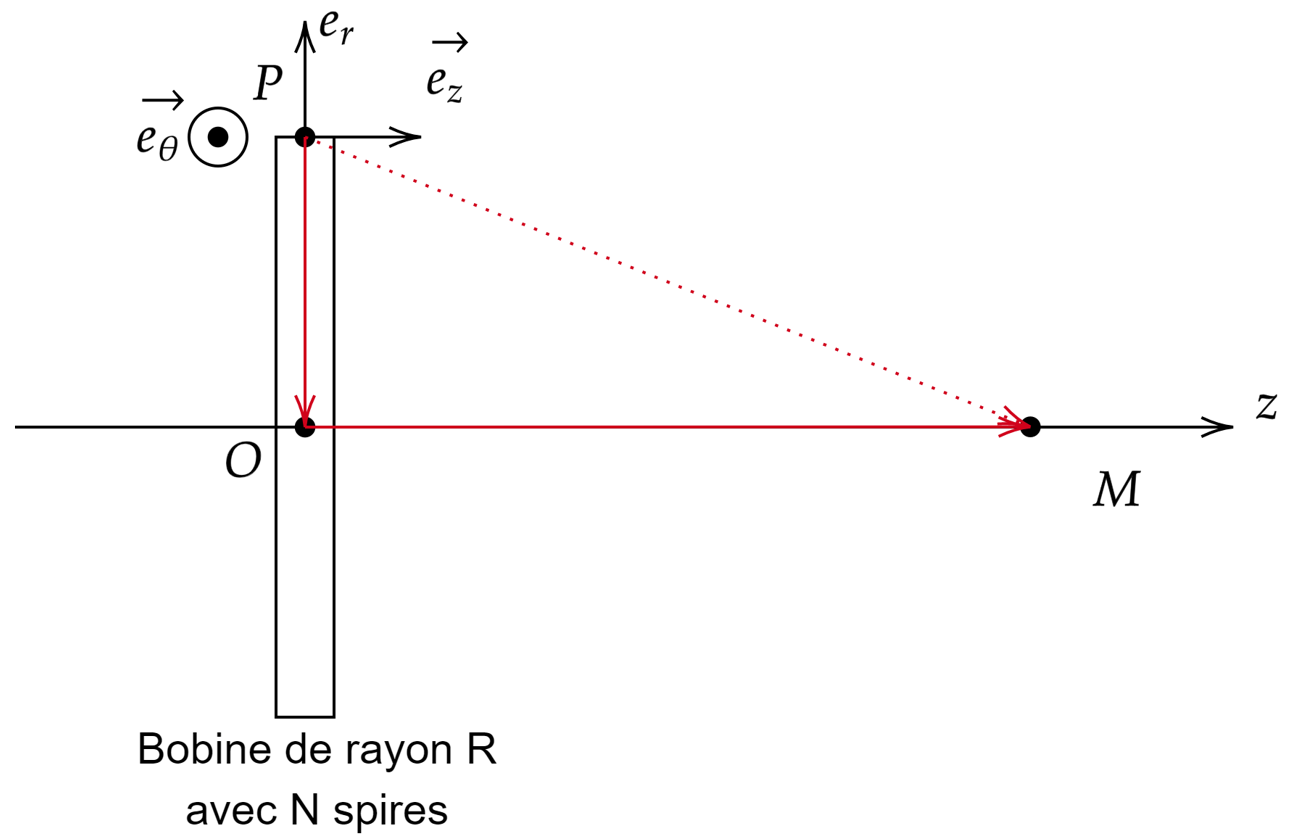
\includegraphics[scale=0.4]{img/theorie.png}
    \end{center}
    \caption{Schéma de la bobine et des différents vecteurs}
\end{figure}

\begin{equation}
    \vec{B}(\vec{r}) = \frac{\mu_0}{4 \pi} \oint_C \frac{I d\vec{l} \wedge (\vec{PM})}{PM^3}
\end{equation}

Sachant que la distance $PM$ est constante lorsque l'on parcoure la spire, et $I$ est constant, on peut les sortir. De plus,
on découpe l'intégrale en deux en notant que $\vec{PM} = \vec{PO} + \vec{OM}$.

\begin{equation}
    \vec{B}(\vec{r}) = \frac{I \mu_0}{4 \pi PM^3} \left( \oint_C d\vec{l} \wedge \vec{PO} + \oint_C d\vec{l} \wedge \vec{OM} \right)
\end{equation}

On exprime les deux intégrales à part:
\begin{gather*}
    \oint_C d\vec{l} \wedge \vec{OM} = \oint_C rd\theta \vec{e_\theta} \wedge z\vec{e_z} = \oint_C rd\theta \vec{e_r} = \vec{0} \\
    \oint_C d\vec{l} \wedge \vec{PO} = \oint_C rd\theta \vec{e_\theta} \wedge r * (-\vec{e_r}) = \oint_C r^2 d\theta \vec{e_z} = 2 \pi r^2\vec{e_z}
\end{gather*}

On a finalement que:
\begin{equation}
    \vec{B}(\vec{r}) = \frac{I \mu_0 r^2}{2 PM^3} \vec{e_z}
\end{equation}

Cependant, on a $PM = \sqrt{r^2 + z^2}$ donc:
\begin{equation}
    \vec{B}(\vec{r}) = \frac{I \mu_0 r^2}{2 \sqrt{r^2 + z^2}^3} \vec{e_z}
\end{equation}

Dans le cas d'une bobine à $N$ spires, on a:
\begin{equation}
    \label{eqn:champ_magn_z}
    \vec{B}(\vec{r}) = \frac{N I \mu_0 r^2}{2 \sqrt{r^2 + z^2}^3} \vec{e_z}
\end{equation}

Lorsqu'on se place dans le centre de la bobine, c'est à dire $z = 0$, on a plus simplement que:
\begin{equation}
    \label{eqn:champ_magn_0}
    \vec{B_0}(\vec{r}) = \frac{NI \mu_0 r^2}{2r} \vec{e_z} = \frac{NI \mu_0}{2r} \vec{e_z}
\end{equation}

\newpage
\subsection{Expérimentation}
Pour cette expérience, on positionne une bobine de $N = 154$ spires et de rayon $r = 20 \pm 0.1 cm$ au centre du banc de telle sorte à pouvoir réaliser
autant de mesures de chaque côté de cette dernière. Avec une source de tension, on alimente la bobine avec 
afin de lui fournir un courant $I = 1.985 \pm 0.005A$.

Pour commencer, on souhaite déterminer l'influence du sens du courant sur le champ magnétique. Pour cela, on suit le protocole
suivant:

\begin{enumerate}
    \item A l'aide d'une boussole, on détermine la direction et le sens du champ magnétique $\vec{B}$, ainsi que les lignes de champs
    en déplaçant la boussole le long de l'axe de la bobine en s'éloignant. \label{etape:boussole}
    \item En prenant soin d'éteindre la source de courant, on inverse le courant et l'on allume de nouveau la source.
    \item On détermine de nouveau l'orientation du champ magnétique avec la boussole en suivant l'étape \ref{etape:boussole}. 
\end{enumerate}

En inversant le courant, on remarque que la boussole pointe dans le sens opposé, mais les lignes de champs restent identiques. On représente
les lignes de champs dans la figure suivante:

\begin{figure}[h!]
    \begin{center}
        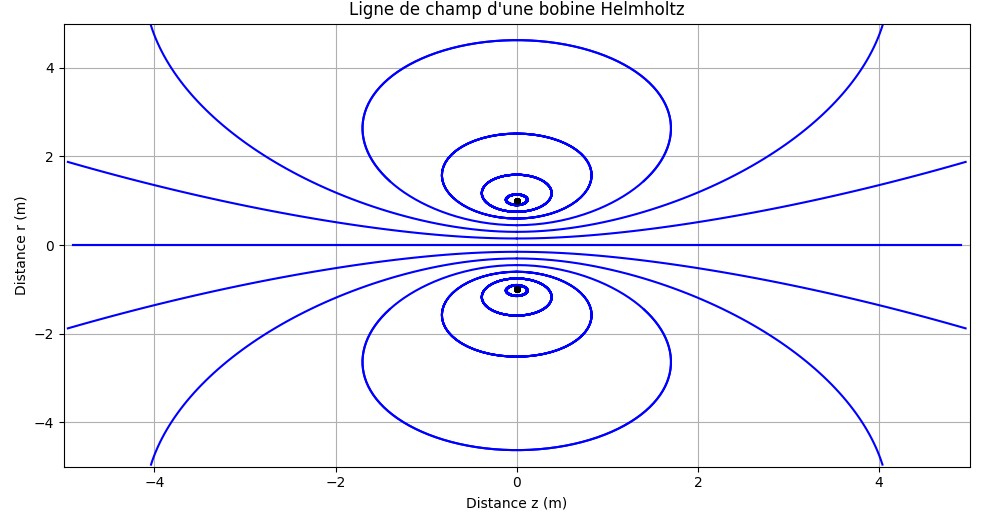
\includegraphics[scale=0.6]{img/LigneChamp.png}
    \end{center}
    \caption{Ligne de champ d'une seule bobine d'Helmholtz}
\end{figure}

\textbf{Remarque:} les lignes de champ et leurs positions ne reflétent pas la réalité, ce graphique a juste pour but de visualiser ces dernières.

\newpage
Ensuite, on détermine l'influence de la distance $z$ avec la bobine sur l'intensité du champ magnétique. Pour cela, avec une sonde de Hall, on mesure l'intensité 
du champ magnétique sur l'axe $Oz$, à différentes distances $z$, en faisant cela de chaque côté de la bobine. Cependant, nous devons déterminer l'intervalle à laquelle nous
allons mesurer le champ magnétique. \\
On remarque que dans l'éqution (\ref{eqn:champ_magn_z}), l'intensité du champ magnétique est inversement proportionnel à $\sqrt{r^2 + z^2}^3$.
On en déduit que l'intensité varie très rapidement lorsque l'on mesure proche du centre de la bobine. Pour pallier à ce problème, on réalisera dans un premier temps 
des mesures tous les 2cm entre $z=0cm$ et $z=20cm$ puis tous les 5cm jusque $z=60cm$.
On trace donc l'intensité de $\vec{B}$ selon la distance $z$ avec la bobine et on observe une intensité maximale au centre de la bobine.

\begin{figure}[h!]
    \begin{center}
        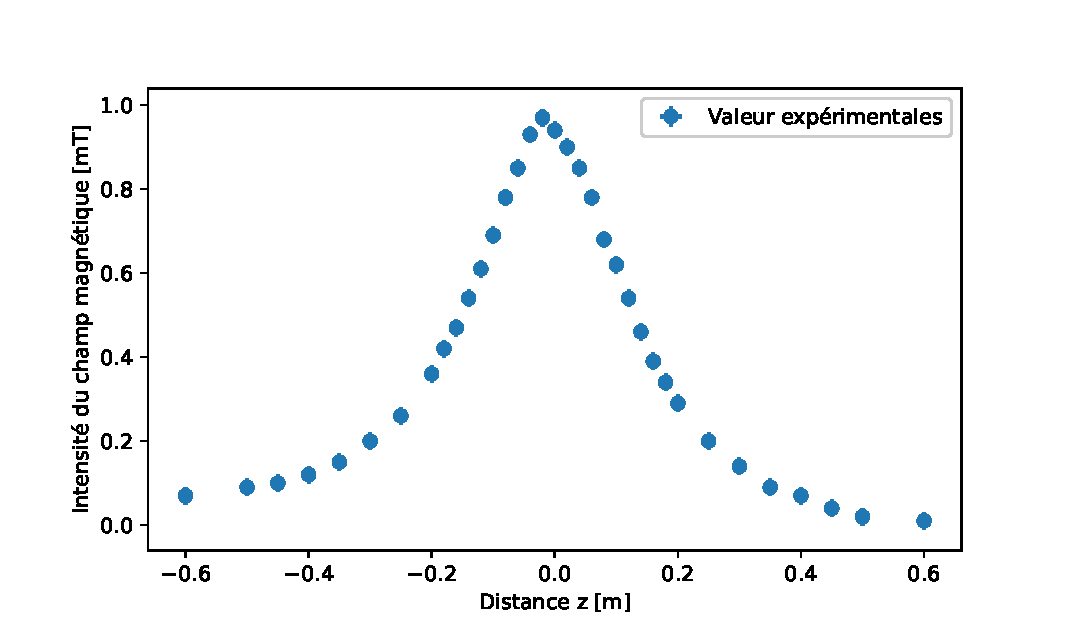
\includegraphics[scale=0.6]{img/MagnEnFonctionDeZ.eps}
    \end{center}
    \caption{Influence de la distance $z$ sur l'intensité du champ magnétique}
\end{figure}

Enfin, on mesure l'effet de l'intensité du courant sur l'intensité du champ magnétique. On positionne donc notre
sonde de Hall (la pointe) au centre de la bobine (ie $z=0m$). On alimente la bobine à différentes tensions, et l'on mesure 
le courant réel parcourant notre bobine avec un ampèremètre et l'intensité du champ magnétique. Selon l'équation (\ref{eqn:champ_magn_0}), 
la relation $B$ et $I$ est affine, on peut donc réaliser des mesures à des courants suffisament espacés.
On trace donc $\norm{\vec{B}}$ en fonction $I$.

\begin{figure}[h!]
    \begin{center}
        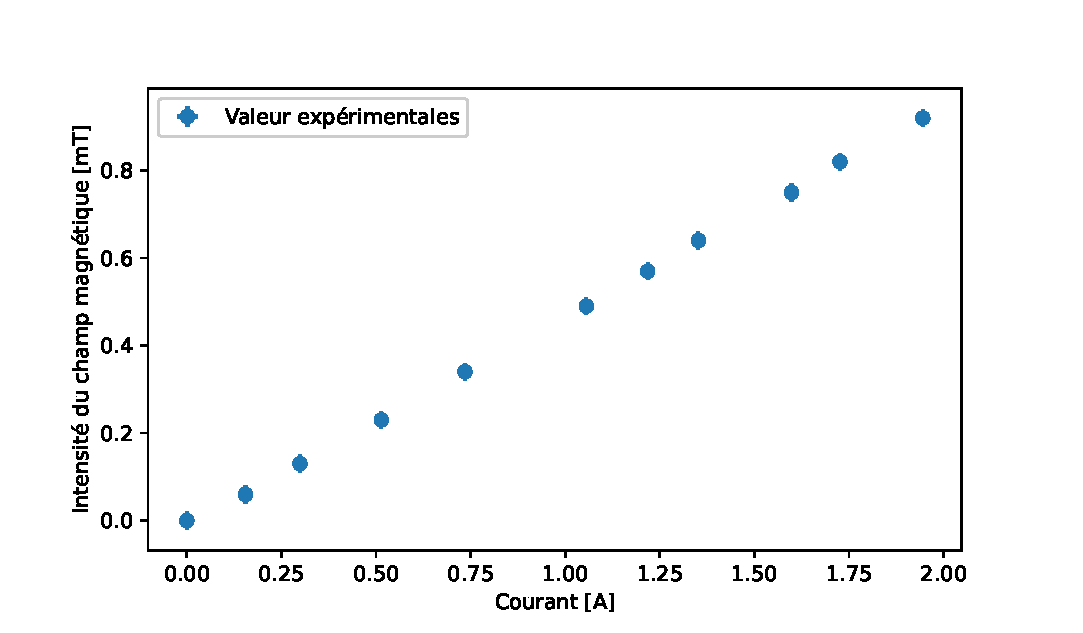
\includegraphics[scale=0.6]{img/MagnEnFonctionDeI.eps}
    \end{center}
    \caption{Influence de l'intensité du courant sur l'intensité du champ magnétique}
\end{figure}

\newpage

\subsection{Modélisation}
Dans cette partie, nous allons comparer nos valeurs expérimentales à la théorie vue en tout premier lieu. Ainsi,
on comparera l'intensité du champ magnétique au centre de la bobine à ce que la théorie prédit, puis on comparera la courbe
de l'intensité du champ magnétique selon $z$ face à l'intensité attendue selon la théorie, tout cela avec un courant $I$ fixe.

On commence par comparer l'intensité du champ magnétique au centre de la bobine, pour cela, on utilisera nos mesures où l'on fait varier le courant dans la bobine.

\begin{figure}[h!]
    \begin{center}
        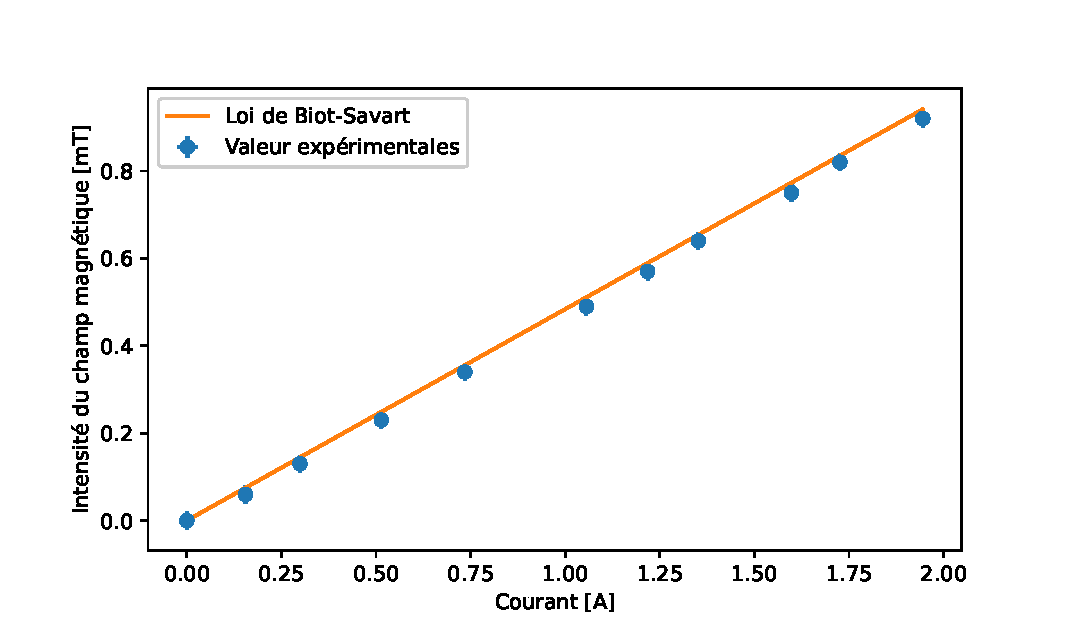
\includegraphics[scale=0.6]{img/ComparaisonBO.eps}
    \end{center}
    \caption{Comparaison de l'intensité du champ entre nos mesures et la valeur prédite par le modèle}
\end{figure}

On remarque de suite que les valeurs prédites par la loi de Biot-Savart sont bien incluses dans nos valeurs expérimentales en prenant en compte les incertitudes. Numériquement, 
on relève un écart relatif maximum avec la valeur théorique de 1\%, ce qui est un écart acceptable dans notre situation. On en conclut donc que la loi de Biot-Savart 
prédit correctement le comportement de l'intensité du champ magnétique au centre de la bobine.

% \begin{align*}
%     \delta B & = \abs{\frac{\partial B}{\partial I}} \delta I + \abs{\frac{\partial B}{\partial r}} \delta r + \abs{\frac{\partial B}{\partial z}} \delta z \\
%     & = \frac{\mu_0}{2} r^2\left(r^2+z^2\right)^{3/2}\delta I \\
%     & + \frac{\mu_0}{2} \left( 2Ir\left(r^2 + z^2\right)^{3/2} + 3I r^3\left(r^2 + z^2\right)^{1/2} \right) \delta r \\
%     & + \frac{\mu_0}{2} 3Ir^2z\left(r^2+z^2\right)^{1/2} \delta z
% \end{align*}

\newpage
On s'intéresse maintenant à l'intensité du champ le long de l'axe $Oz$, on trace donc la courbe prédite par la loi de Biot-Savart, par dessus la courbe que l'on a obtenu précédemment.
\begin{figure}[h!]
    \begin{center}
        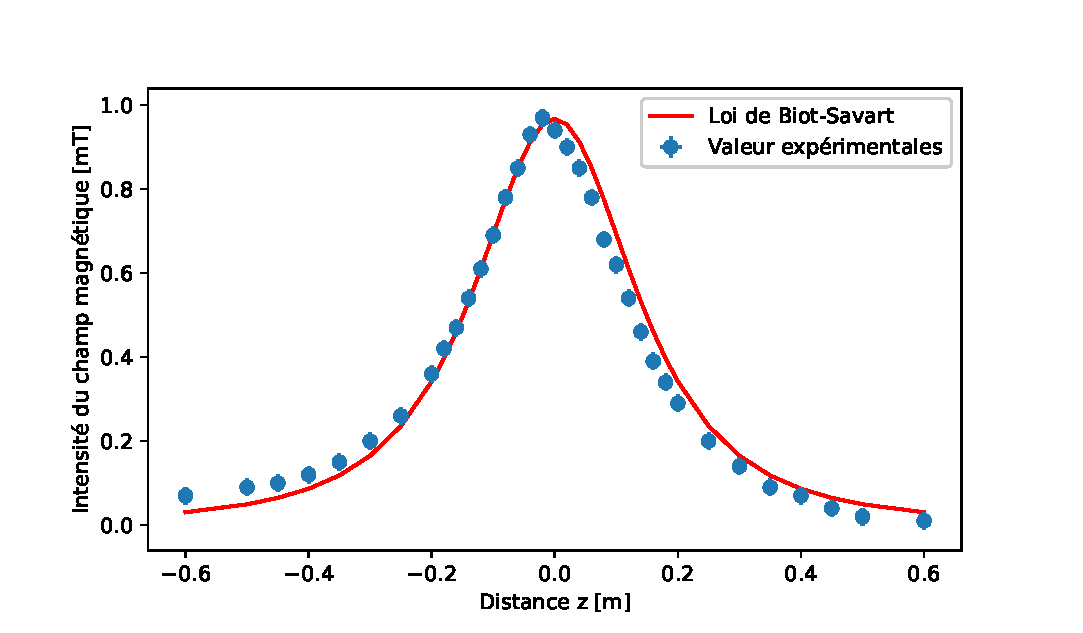
\includegraphics[scale=0.6]{img/ComparaisonB.eps}
    \end{center}
    \caption{Comparaison de l'intensité du champ entre nos mesures et la valeur prédite par le modèle}
\end{figure}
\newpage

\section{Montage avec deux bobines}
On souhaite cette fois vérifier la loi de Biot-Savart avec un montage avec deux bobines espacées d'une distance $d$. On doit donc chercher le centre de ces deux bobines où 
l'intensité du champ magnétique est nulle. On cherche donc la configuration présentant une intensité nulle à un point entre les deux bobines.

\begin{figure}[h!]
    \centering
    \subfloat[Intensité du champ magnétique]{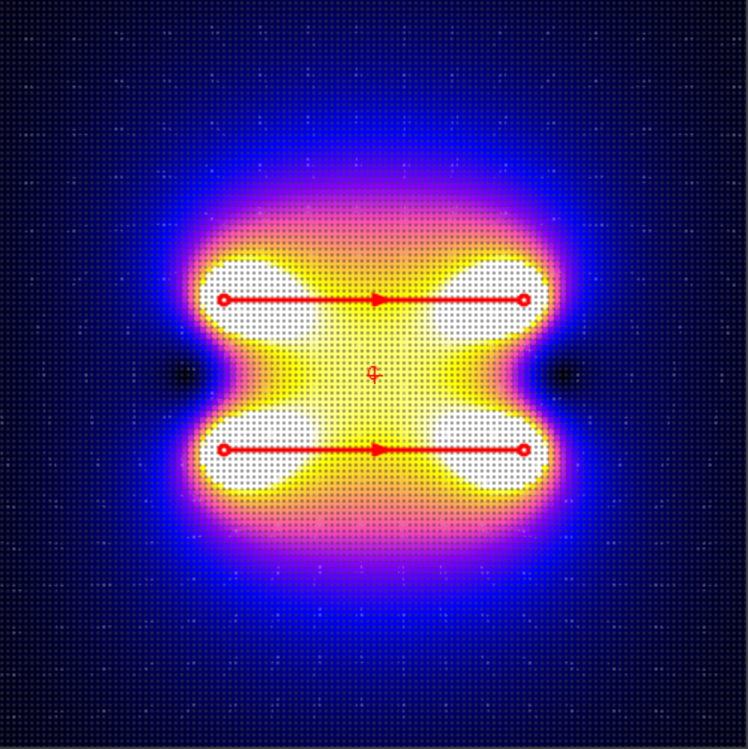
\includegraphics[width=0.35\textwidth]{img/HelmIntensite.png}}
    \quad \quad
    \subfloat[Champ magnétique]{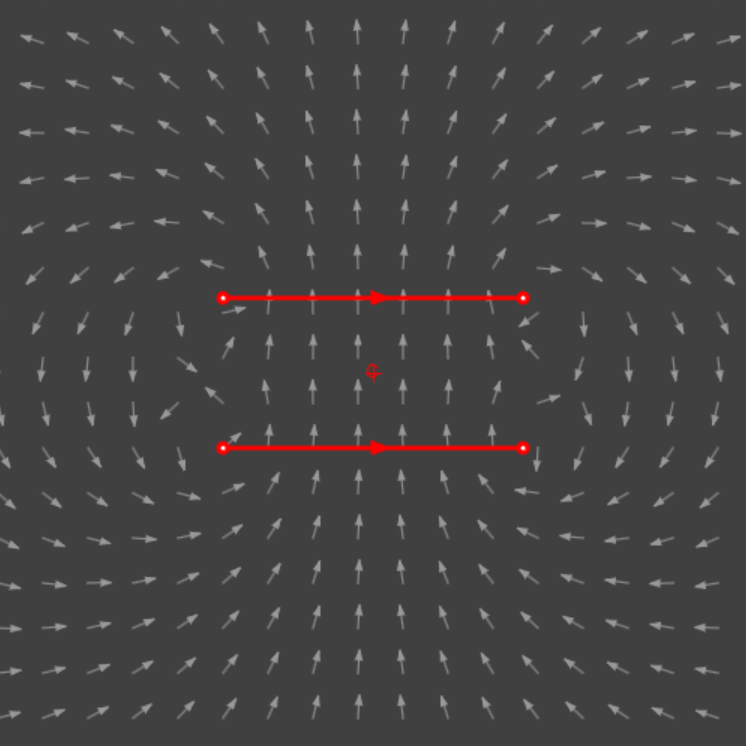
\includegraphics[width=0.35\textwidth]{img/HelmVect.png}}
    \caption{Champ magnétique dans le cas de bobine alimenté par un courant dans le même sens (vu du dessus) (Source: FemtoPhysique)}
\end{figure}

\begin{figure}[h!]
    \centering
    \subfloat[Intensité du champ magnétique]{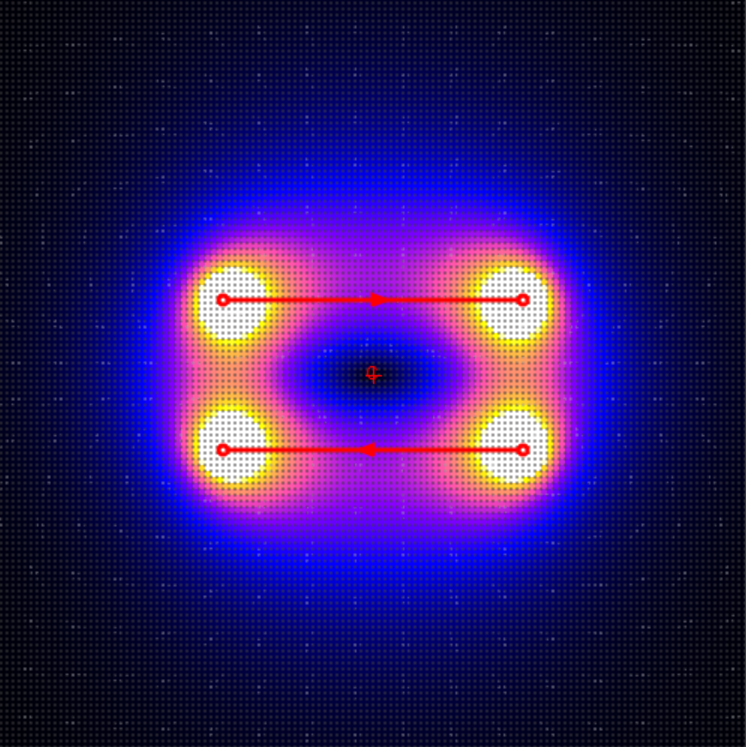
\includegraphics[width=0.35\textwidth]{img/HelmAntiIntensite.png}}
    \quad \quad
    \subfloat[Champ magnétique]{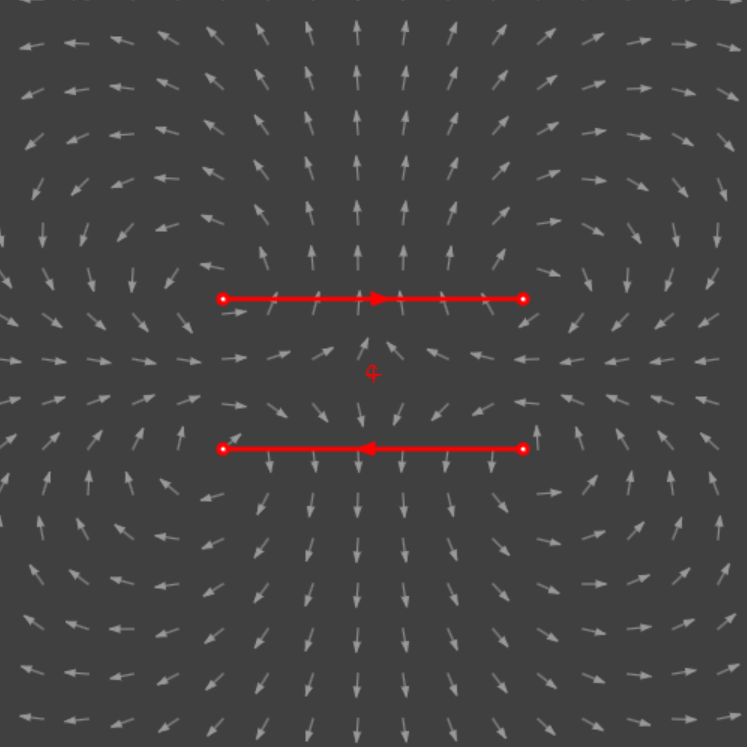
\includegraphics[width=0.35\textwidth]{img/HelmAntiVect.png}}
    \caption{Champ magnétique dans le cas de bobine alimenté par des courants opposés (vu du dessus) (Source: FemtoPhysique)}
\end{figure}
Sur les figures ci-dessus, plus la couleur est noire, plus l'intensité est faible, plus c'est blanc, plus l'intensité est grande. On remarque ainsi que dans le cas d'une configuration
où les deux bobines sont parcourues par un courant de sens opposé, le champ magnétique présente un point central d'intensité nulle, ce qu'on observe pas dans le cas avec un courant 
parcourant les deux bobines dans le même sens. Pour déterminer ce point, on placera donc les bobines afin qu'elles générent un champ magnétique qui s'oppose, qui peut donc potentiellement s'annuler en un point.

Ainsi, en sachant qu'une telle configuration présente une intensité nulle au centre des deux bobines, on pourra chercher ce point en déplaçant notre sonde jusqu'à trouver une 
intensité nulle. Une fois cela réalisé, on pourra positionner les bobines pour qu'elles générent un champ magnétique dans le même sens (donc une intensité non nulle au centre). 

Dans la première partie de ce travail pratique, nous avons mesuré l'intensité du champ le long de l'axe $Oz$. Nous allons répéter cette mesure 3 fois en espacant les bobines d'une distance $d$
de 10cm, 20cm puis 50cm et l'on observera la forme du champ magnétique. On obtient donc les trois graphiques suivant:

\begin{figure}[h!]
    \begin{center}
        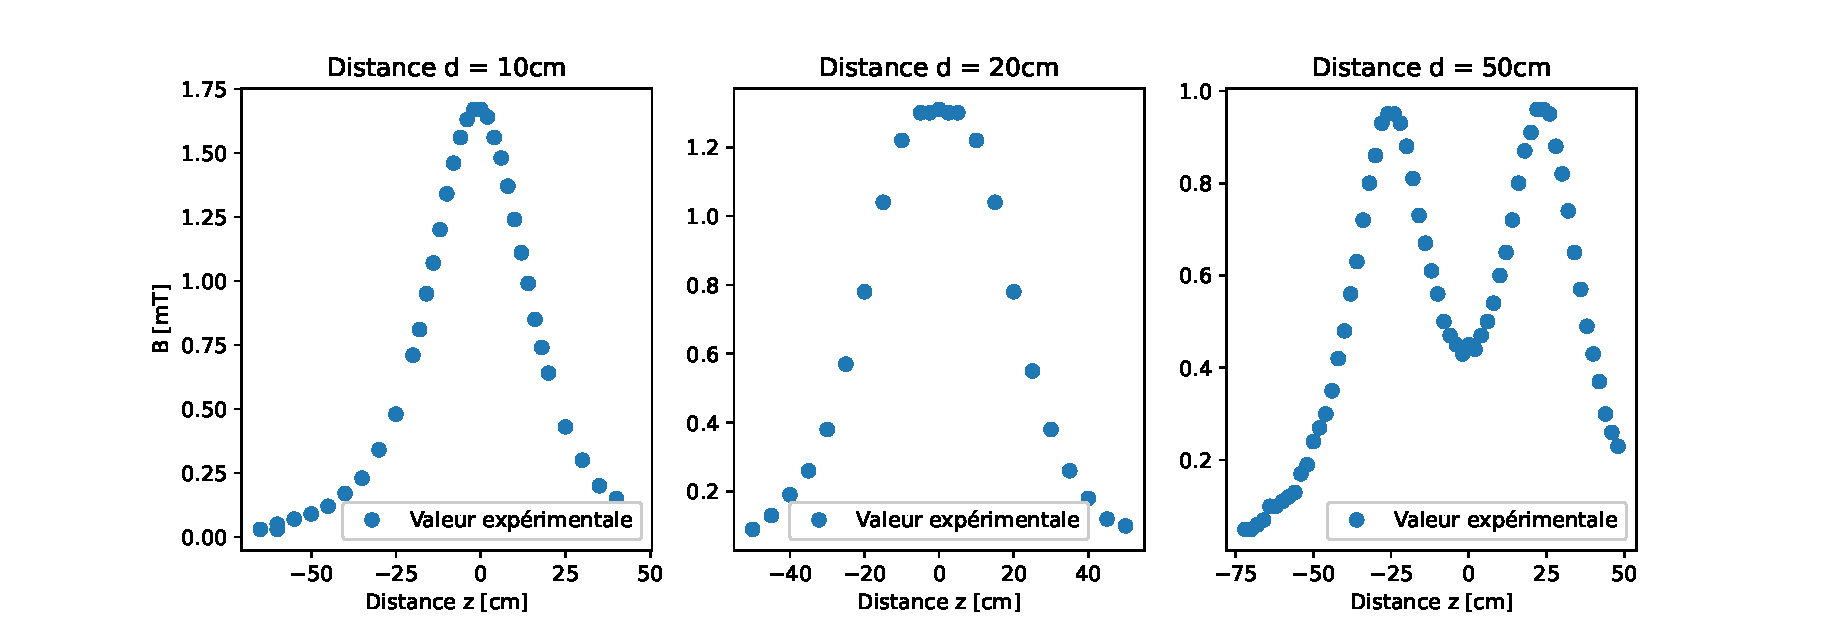
\includegraphics[scale=0.6]{img/ChampDistance.eps}
    \end{center}
    \caption{Comparaison de l'intensité du champ selon l'écart entre les bobines}
\end{figure}

On reporte dans le tableau suivant les intensités maximales et minimales relevées entre les deux bobines pour chaque distance $d$ et l'on calcule la variation relative du champ magnétique
$\frac{\Delta B}{B} = \frac{B_{max} - B_{min}}{B_{min}}$ :

\begin{table}[h!]
    \begin{center}
        \begin{tabular}{c|c|c|c}
            Distance $d$ (en cm) & $B_{min} \pm 0.02$ (en mT) & $B_{max} \pm 0.02$ (en mT) & $\frac{\Delta B}{B} (en \%)$ \\ \hline
            10cm & 1.37 & 1.67 & 22.0 \\
            20cm & 1.22 & 1.31 & 7.40 \\
            50 cm & 0.43 & 0.96 & 123 \\
        \end{tabular}
    \end{center}
\end{table}

On remarque que la variation relative du champ magnétique est très grande lorsque l'on écarte les deux bobines d'une distance $d=50cm$ avec des intensités doublées (voire plus) entre les deux bobines. 
On retrouve un constat similaire avec $d=10cm$, la variation reste marquée entre les deux bobines avec une variation de $22\%$. Cependant, lorsque l'on positionne les deux bobines à une distance $d = 20cm$,
c'est à dire lorsqu'on les écartent avec une distance équivalente à leurs rayons, la variation d'intensité est bien plus faible, avec seulement 7.40\%. Ainsi, la configuration présentant 
le champ le plus uniforme est celle avec une distance $d=20cm$.

On en conclut donc que si l'on souhaite générer un champ magnétique le plus uniforme, il est préférable d'écarter les deux bobines avec une distance équivalente à leurs rayons.

\newpage

\section{Mesure du champ magnétique local}

Le but de cette expérience est de déterminer la valeur du champ magnétique local. On utilise pour cela une boussole et un montage similaire au précédent. 

\subsection{Expérimentation}
On réalise le même montage que l'expérience, avec deux bobines. On écarte nos deux bobines de $70cm$. On commence par faire passer le courant dans un sens opposés. On trouve alors un $z_0$ à l'endroit où le champ magnétique est nul, ce qu'on détermine grâce au Teslamètre. 

On fait ensuite passer le courant dans le même sens dans les deux bobines, et on mesure la valeur du champ magnétique pour différentes valeurs d'intensité, ce qui nous permettra de trouver une relation entre $B$ et $I$. 

On place ensuite notre boussole en $z_0$, et on mesure l'angle $\alpha_0$ que fait la boussole avec l'axe des bobines, lorsque l'intensité est nulle. On installe ensuite le rhéostat en série dans notre montage. On fait varier la valeur de $I$ grâce au rhéostat jusqu'à ce que $\alpha_0$ soit divisé par 2. On note cette intensité $I_l$. 

On regroupe nos données : 
\begin{figure}[!h]
	\begin{center}
		\begin{tabular}{|c|c|}
		\hline
		$I\pm 0.001 \, A$ & $B\pm 0.02\, mT$ \\
		\hline
	$0.0$ & $0.0$ \\ 
$0.246$ & $0.01$ \\ 
$0.592$ & $0.05$ \\ 
$0.882$ & $0.08$ \\ 
$1.154$ & $0.12$ \\ 
$1.436$ & $0.15$ \\ 
$1.69$ & $0.17$ \\ 
$1.998$ & $0.21$ \\ 
	\hline	
		\end{tabular}
	\end{center}
	\label{RelationIB}
	\caption{Valeur du champ magnétique pour différents courants}
\end{figure}

On mesure également: $\alpha_0=57\pm 1^\circ  $,$I_l=0.095\pm 0.001\, A$.

\newpage
\subsection{Modélisation}

On commence par déterminer la relation entre B et I. Les données obtenues permettent de tracer B en fonction de I.
\begin{figure}[!h]
	\begin{center}	
		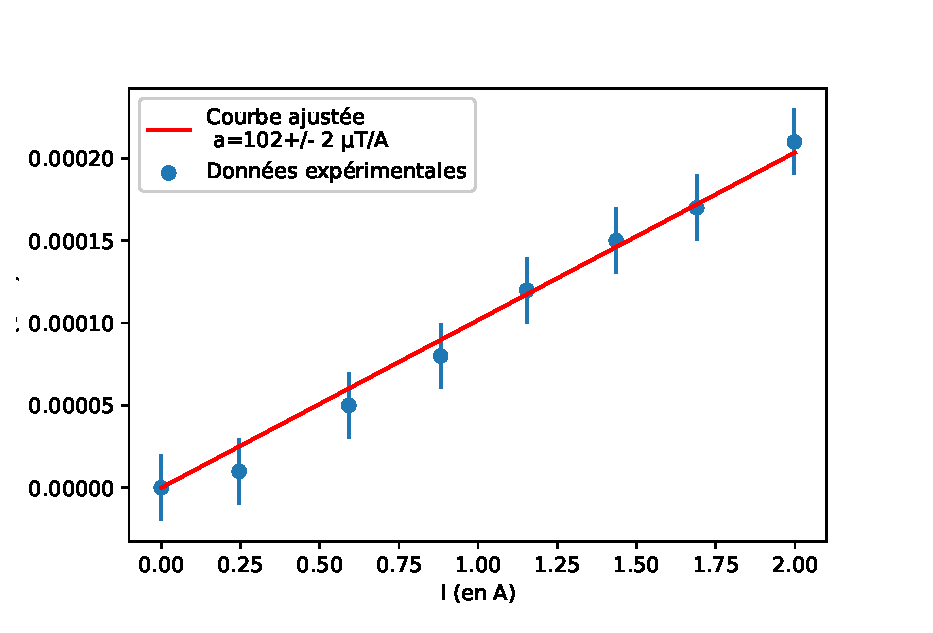
\includegraphics[scale=1]{img/B_fonction_I.eps}
	\end{center}
	\label{BfonctionI}
	\caption{Relation entre le champ magnétique des bobines B et l'intensité I}
\end{figure}

On obtient donc une droite et la relation $B=aI$, avec $a=102\pm 2 \, \mu T/A$.

On cherche maintenant un $I$ tel que $B_{bobine}=B_{local}$. Les bobines créent un champ dans l'axe de la boussole, donc s'il n'y avait pas de champ local mais seulement le champ des bobines, on aurait $\alpha = 0$. 
Inversement, lorsque qu'il n'y a que le champ local, la boussole fait un angle $\alpha_0$ avec l'axe des bobines. 

\newpage
On remarque donc que lorsque le champ local et le champ des bobines ont la même norme, alors la boussole fait un angle $\frac{\alpha_0}{2}$ avec l'axe des bobines. 

\begin{figure}[!h]
	\begin{center}
		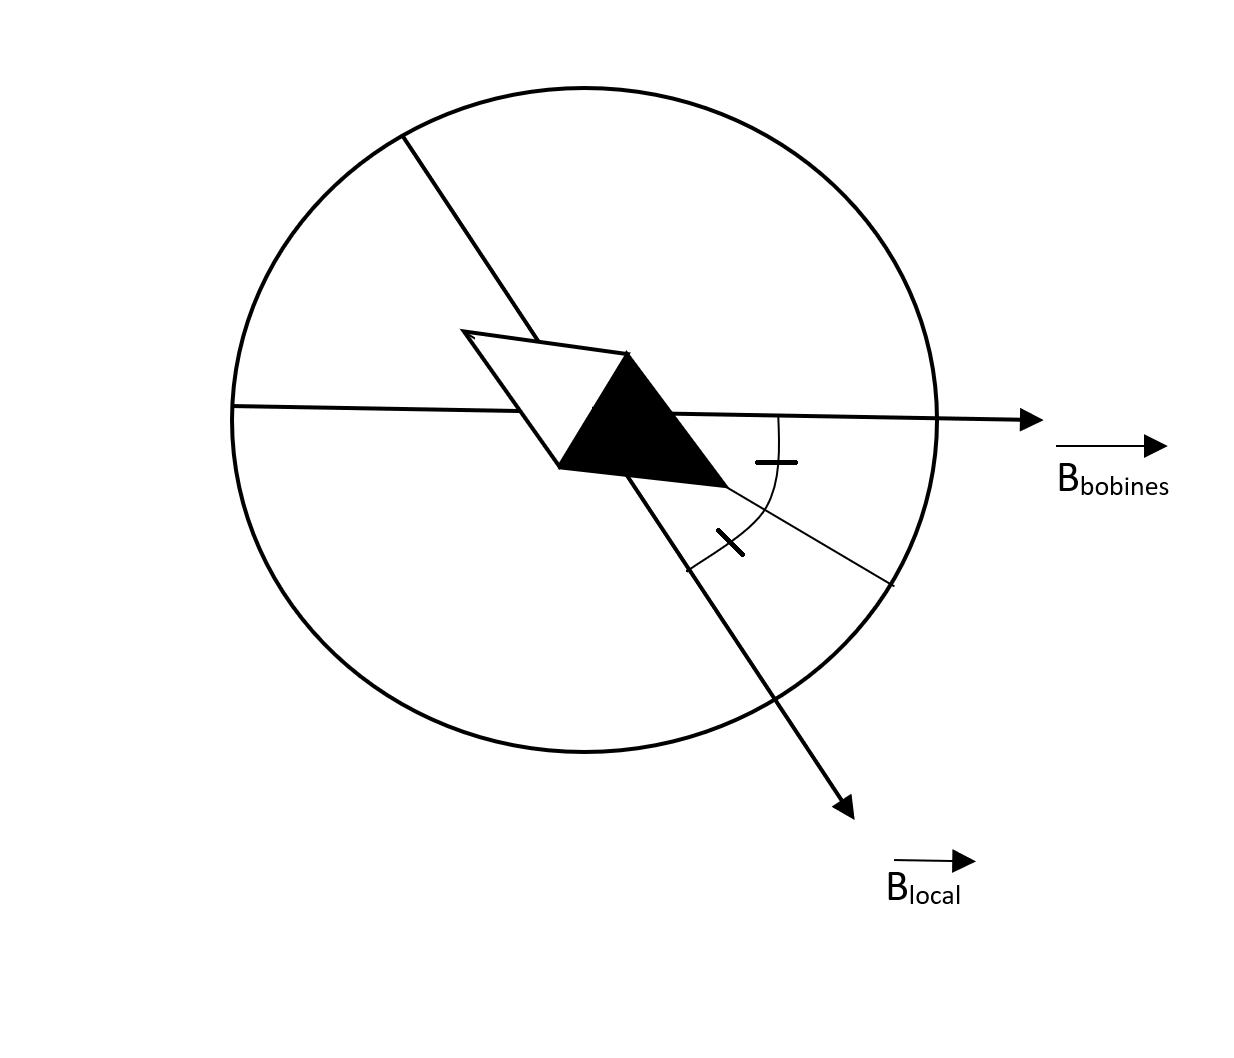
\includegraphics[scale=0.5]{img/Boussole.png}
	\end{center}
	\label{SchmBouss}
	\caption{Schéma de la boussole lorsque $B_{bobines}=B_{local}$}
\end{figure}

Notre $I_l$ mesuré lors de l'expérience est donc la valeur de l'intensité pour laquelle $B_{bobines}=B_{local}$. On a donc:
\begin{align*}
B_{local}&=a*I_l & \delta B_{local}=a*\delta I_l + I_l * \delta a
\end{align*}
On fait l'application numérique et on obtient $B_{local}=9.7\pm 0.3\, \mu T$. Le valeur théorique du champ terrestre est de $47\mu T$. Cette valeur n'est pas comprise dans notre intervalle expérimental et nous avons un écart relatif de 80%. Néanmoins, on peut chercher à déterminer si notre expérience est sensible aux erreurs de mesures. Pour cela, on réalise la même expérience mais en $z=z_0 +1\, cm$.
On détermine de nouveau la mesure entre B et I. On trouve $B=a*I$ avec $a=370\pm 70 \mu T$. 

On mesure cette fois $I_l=0.100\pm 0.001 \, A$. On a donc $B_{local}=37\pm 7 \mu T$. On remarque donc que notre valeur a presque été multipliée par 4 avec un décalage de $4\, cm$. De plus, on a sous-estimé notre incertitude sur $I_l$, car notre boussole n'est pas précise. Dans notre cas,nous avions $\alpha_0=57\pm 1^\circ$. Il aurait donc fallu mesurer $I_{min}$ à $29^\circ$ et $I_{max}$ à $28^\circ$. On aurait alors eu une incertitude plus réaliste. 

\newpage
\section*{Conclusion}

Dans ce travail pratique, nous avons commencé par étudier la champ magnétique crée par une bobine parcouru par un courant électrique. Nous avons commencé par déterminer le sens et la direction du champ magnétique grâce à une boussole. Puis nous avons calculé la valeur de ce champ le long de l'axe de la bobine et pour différentes valeurs de courant. Les résultats obtenus sont cohérents avec la loi de Biot-Savart. 

Nous avons ensuite étudié un montage avec deux bobines. Nous nous somme intéressés à l'homogénéité du champ crée par les bobines en fonction de la distance qui les sépare. Nous avons conclus que le champ était le plus homogène lorsque les bobines étaient séparées par une distance équivalente à leurs rayons. 

Enfin, nous avons déterminer la valeur du champ magnétique local grâce à deux bobines et une boussole. La valeur obtenue était du même ordre de grandeur que la valeur théorique, de l'ordre du microTesla, mais nous n'avons pas pu retrouver exactement la même valeur. Pour améliorer notre protocole, il faudrait mieux prendre en compte l'incertitude sur la boussole, en prenant un plus grand intervalle pour le courant qui engendre le champ des bobines. Cela nous permettrait d'avoir une incertitude plus réaliste sur notre valeur finale du champ magnétique locale. 

\end{document}
